% !TEX root =  bopp.tex


\begin{figure}[t]
	\begin{lstlisting}[basicstyle=\footnotesize\ttfamily]
(defopt mvn-mixture [data mu0 kappa psi] [nu alpha]
 (let [[n d] (shape data)
       alpha (sample (uniform-continuous 0.01 100))
       nu (sample (uniform-continuous (- d 1) 100))
       obs-proc0 (mvn-niw mu0 kappa nu psi)]
       (loop [data data
              obs-procs {}
              mix-proc (dirichlet-discrete 
                          (vec (repeat d alpha)))]
	    (let [y (first data)]
	     (if y
	      (let [z (sample (produce comp-proc))
	            obs-proc (get obs-procs z obs-proc0)
	            obs-dist (produce obs-proc)]
	        (observe obs-dist y)
	        (recur (rest data)
	               (assoc obs-procs z (absorb obs-proc y))
	        (absorb mix-proc z)))
	      mix-proc)))))
	\end{lstlisting}
	\caption{
		\label{fig:mvn-code}
		Anglican query for hyperparameter optimization of a Gaussian mixture model, defined in terms of two parameters \lsi{nu} and \lsi{alpha}. A \lsi{mvn-niw} process is used to represent the marginal likelihood of observations under a Gaussian-inverse-Wishart prior, whereas a \lsi{dirichlet-discrete} process models the prior probability of cluster assignments under a Dirichlet-discrete prior. The command \lsi{produce} returns the predictive distribution for the next sample from a process. \lsi{absorb} conditions on the value of the next sample.}
\end{figure}

\begin{figure*}[t]
	%	\includegraphics[width=1.7in]{"../figures/mvn-mixture/opt-nu-alpha-160229-01-10"}
	%	~
	%	\includegraphics[width=1.7in]{"../figures/mvn-mixture/opt-nu-alpha-160229-01-20"}
	%	~
	%	\includegraphics[width=1.7in]{"../figures/mvn-mixture/opt-nu-alpha-160229-01-50"}
	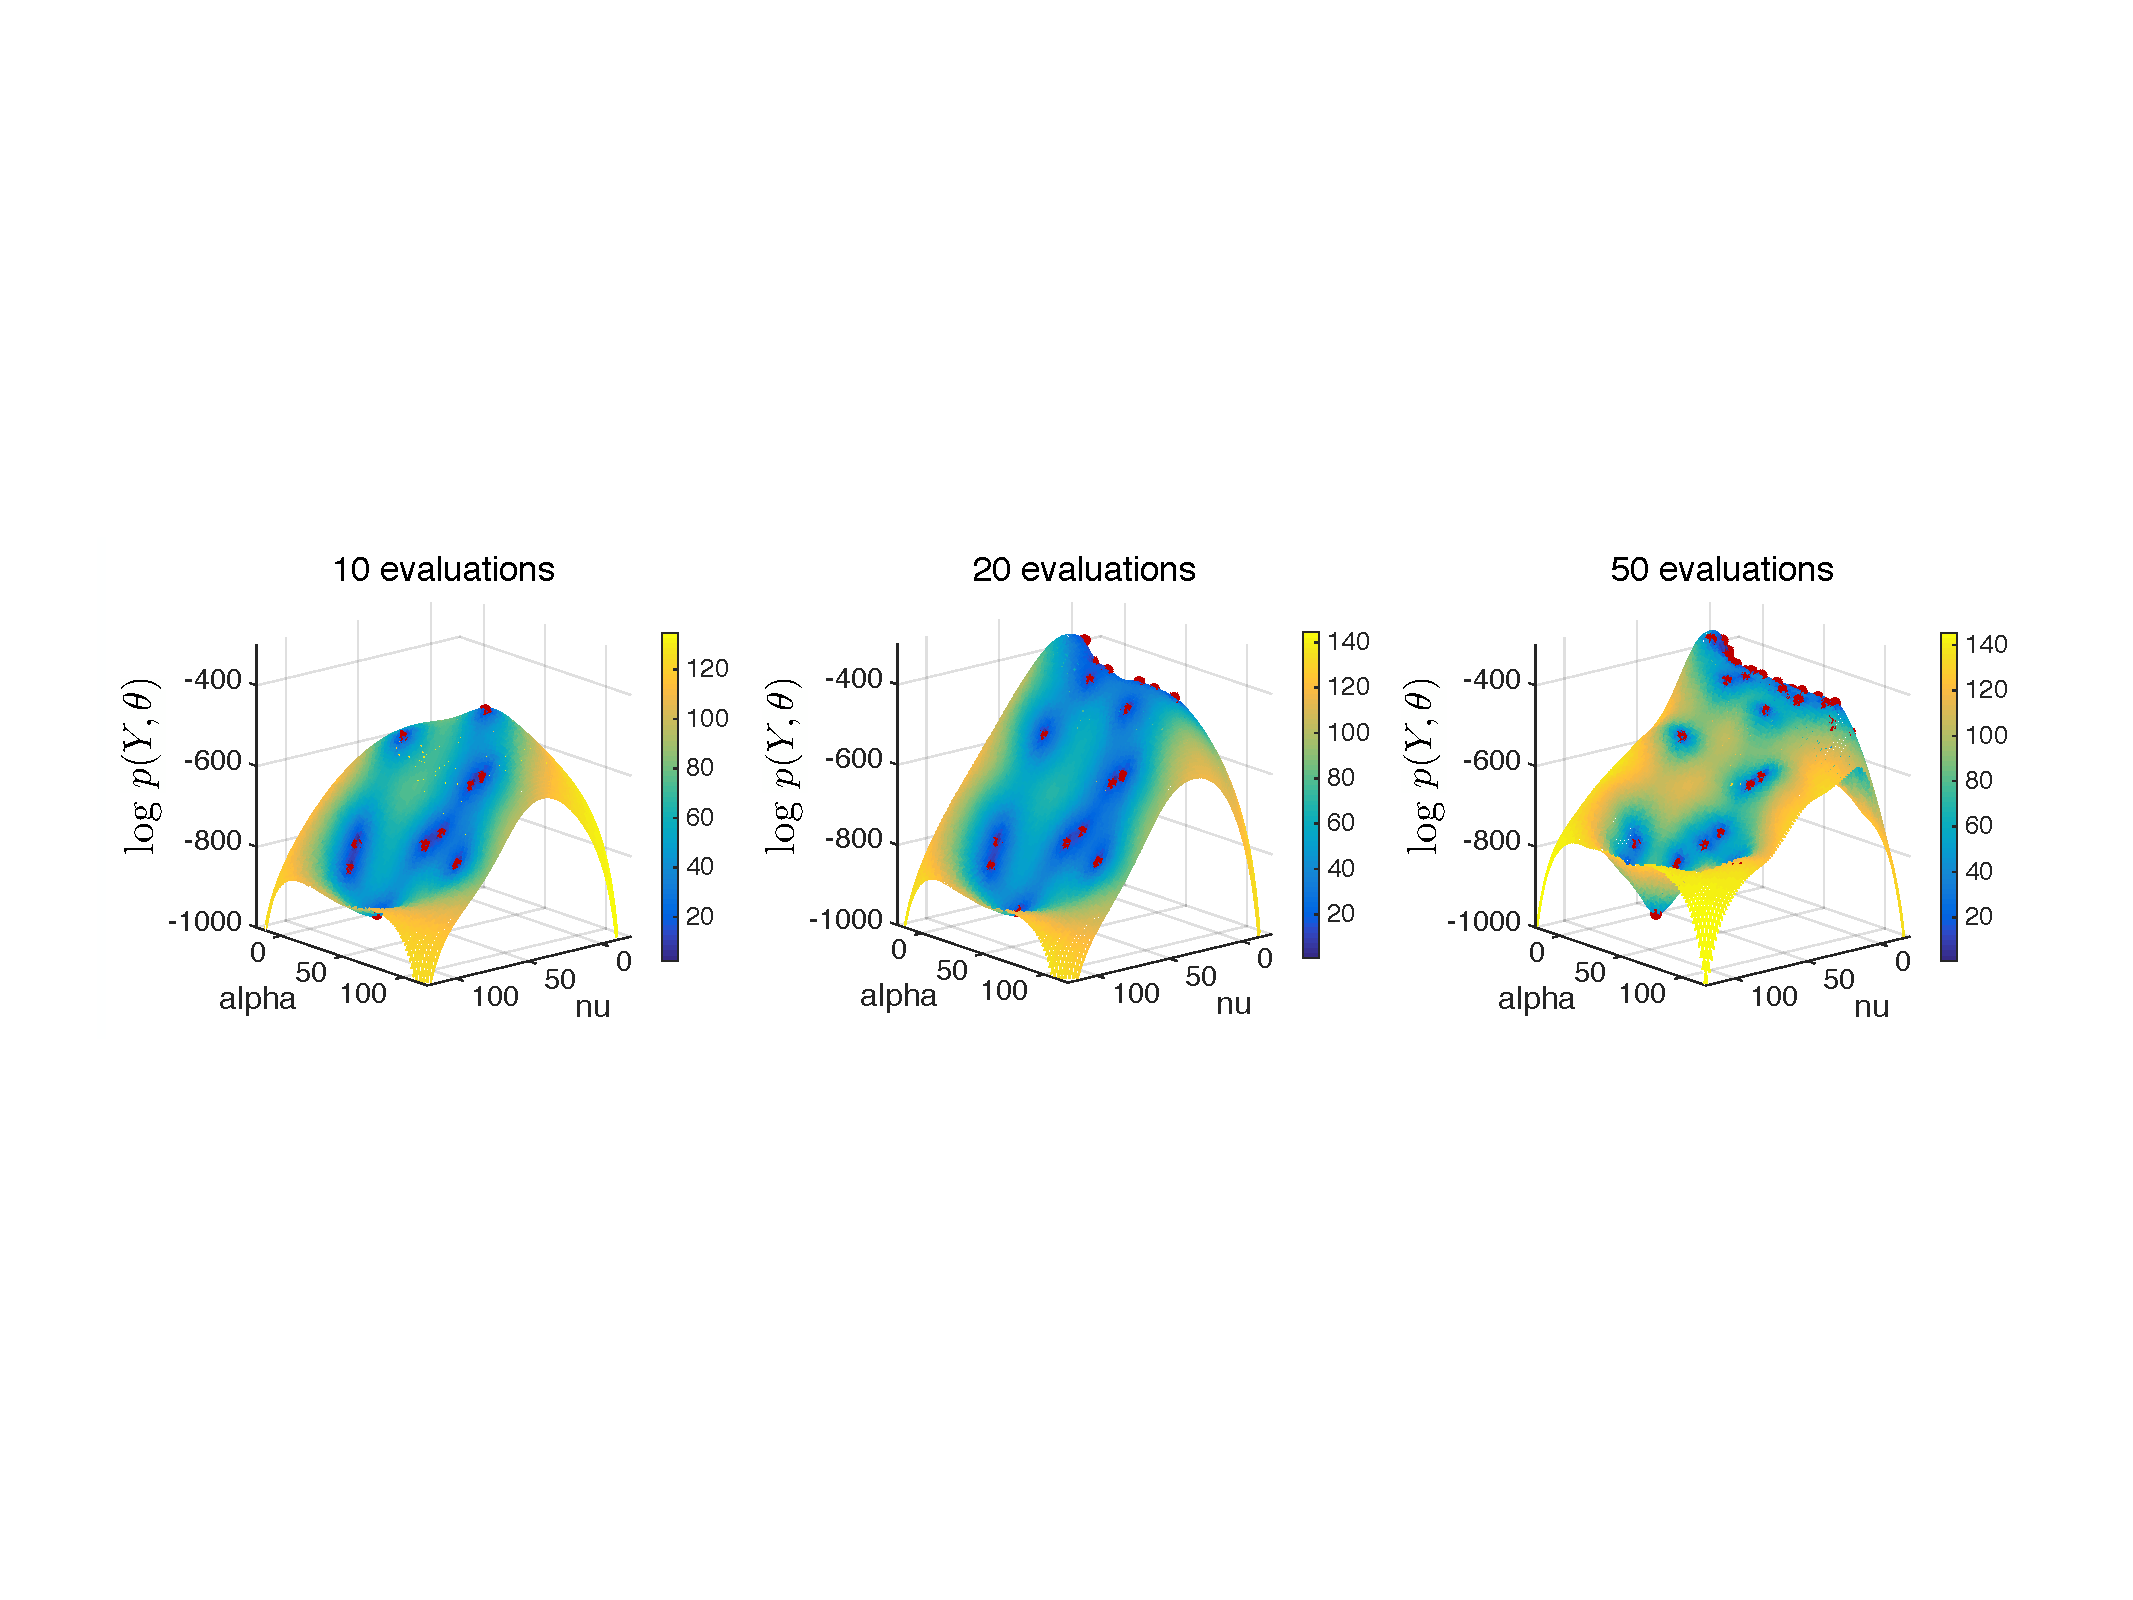
\includegraphics[width=\textwidth]{mvn-mixture/axis_corr_mvn_gps}
	\caption{
		\label{fig:mvn-gp-surface}
		Bayesian optimization of hyperparameters in a Gaussian mixture model evaluated on the Iris dataset. Panels show the GP posterior as a function of number of evaluations, with the surface corresponding to the posterior mean and the color bars the posterior standard deviation. Optimization is performed over the parameter $\alpha$ of a 10-dimensional symmetric Dirichlet distribution and the degrees of freedom $\nu$ of the inverse-Wishart prior. At each evaluation we obtain an estimate of the log marginal $\log p(Y,\theta)$ obtained by performing sequential Monte Carlo inference with 1000 particles.  The apparent maximum after initialization with 10 randomly sampled points lies at $\nu=31$, $\alpha=60$, and $\log p(Y,\theta) = -456.3$ (\emph{left}).  The surface after 10 optimization steps shows a new maximum at $\nu=9.2$, $\alpha=0.8$, and $\log p(Y,\theta) = -364.2$ (\emph{middle}). After 40 steps and 50 total evaluations this optimum is refined to $\nu=16$, $\alpha = 0.2$, and $\log p(Y,\theta) = -352.5$  (\emph{right}).}
\end{figure*}

We start with an illustrative case study of optimizing the hyperparameters in a multivariate Gaussian mixture model. We consider a Bayesian formulation with a symmetric Dirichlet prior on the mixture weights and a Gaussian-inverse-Wishart prior on the likelihood parameters:
\begin{align}
\v{\pi}
&\sim 
{\rm Dir(\alpha, \ldots, \alpha)}
\displaybreak[0]\\
(\v{\mu}_k, \v{\Sigma}_k)
&\sim 
{\rm NIW} (\v{\mu}_0, \kappa, \v{\Psi}, \nu)
&
{\rm for~}
&
k = 1, \ldots , K
\displaybreak[0]\\
z_n 
&\sim 
{\rm Disc(\v{\pi})}
\displaybreak[0]\\
\v{y}_n
&
\sim
{\rm Norm}(\v{\mu}_{z_n}, \v{\Sigma}_{z_n})
&
{\rm for~}
&
n = 1, \ldots , N
\end{align}
% Figure~\ref{fig:mvn-code} shows an optimization query for an Anglican program corresponding to this model. 
Anglican code for this model is shown in Figure 4. Anglican provides stateful objects, which are referred to as random processes, to represent the predictive distributions for the cluster assignments $z$ and the observations $\v{y}^k$ assigned to each cluster
\begin{align}
z_{n+1}
& \sim 
p( \cdot \,|\, z_{1:n}, \alpha),
\\
\v{y}_{m+1}^{k} 
& \sim 
p(\cdot \,|\, \v{y}^k_{1:m}, \v{\mu}_0, \kappa, \v{\Psi}, \nu).
\end{align}
In this collapsed representation marginalization over the model parameters $\v{\pi}$, $\v{\mu}_{k=1:K}$, and $\v{\Sigma}_{k=1:K}$ is performed analytically.
%The only variables that are sampled during program execution are the cluster assignments $z_{1:N}$, which we marginalize over using the general-purpose sequential Monte Carlo (SMC) implementation provided by the inference back end. 
%Like any importance sampling method, SMC provides an unbiased estimate $\hat Z$ of the marginal likelihood $Z = p(\v{y}_{1:N} | \alpha, \v{\mu}, \kappa, \v{\Psi}, \nu)$. 
%Intuitively, the parameter $\nu$, which is known as the degrees of freedom, represents a scale factor for the covariance matrix, which determines the spatial extent of the clusters (larger $\nu$ values imply a smaller covariance and cluster size). 
%The parameter $\alpha$, sometimes known as a concentration parameter, controls the distribution on mixture weights (where $\alpha \gg 1.0$ implies an even distribution and $\alpha \ll 1.0$ implies an uneven distribution).  
Using the Iris dataset, a standard benchmark for mixture models that contains 150 labeled examples with 4 real-valued features, we optimize the marginal with respect to the subset of the parameters $\nu$ and $\alpha$ under uniform priors over a fixed interval.  For this model, BOPP aims to maximize
\begin{align}
\begin{split}
& p(\nu, \alpha | \v{y}_{n=1:N}, \v{\mu}_0, \kappa, \v{\Psi}) \\
&= \iiiint p(\nu, \alpha, z_{n=1:N}, \v{\pi}, \v{\mu}_{k=1:K}, \v{\Sigma}_{k=1:K} | \v{y}_{n=1:N}, \mu_0, \kappa, \v{\Psi}) \mathrm{d}z_{n=1:N}\mathrm{d}\v{\pi}\mathrm{d}\v{\mu}_{k=1:K}\mathrm{d}\v{\Sigma}_{k=1:K}.
\end{split}
\end{align}

Figure~\ref{fig:mvn-gp-surface} shows GP regressions on the evidence after different numbers of the SMC evaluations have been performed on the model.  This demonstrates how the GP surrogate used by BO builds up a model of the target, used to both estimate the expected value of $\log p(Y,\theta)$ for a particular $\theta$ and actively sample the $\theta$ at which to undertake inference.

% n=10
% x1_max: 30.90
% x2_max: 61.55
% y_max: -456.32
% mu_max: -456.33
% sig_max: 0.51

% n=20
% x1_max: 9.20
% x2_max: 0.79
% y_max: -364.21
% mu_max: -364.23
% sig_max: 0.47

% n=50
% x1_max: 16.34
% x2_max: 0.21
% y_max: -352.51
% mu_max: -352.51
% sig_max: 0.53

% n=100
% x1_max: 16.34
% x2_max: 0.21
% y_max: -352.51
% mu_max: -352.50
% sig_max: 0.41

% \begin{figure}
% \begin{lstlisting}[basicstyle=\footnotesize\ttfamily]
% (defopt mvn-mixture 
%  [data mu kappa psi] [:nu :alpha]
%  (let [[n d] (shape data)
%        alpha (sample :alpha
%               (uniform-continuous 0.01 100))
%        nu (sample :nu 
%            (uniform-continuous (- d 1) 100))
%        obs-proc0 (mvn-niw mu kappa nu psi)]
%   (loop [data data
%          obs-procs {}
%          mix-proc (dirichlet-discrete 
%                    (vec (repeat d alpha)))]
%    (let [y (first data)]
%     (if y
%      (let [z (sample (produce comp-proc))
%            obs-proc (get obs-procs 
%                      z obs-proc0)
%            obs-dist (produce obs-proc)]
%       (observe obs-dist y)
%       (recur (rest data)
%              (assoc obs-procs
%                z (absorb obs-proc y))
%              (absorb mix-proc z)))
%      (predict mix-proc))))))
% \end{lstlisting}
% \caption{
% \label{fig:mvn-code}
% Anglican query for hyperparameter optimization of a Gaussian mixture model, defined in terms of two parameters \lsi{:nu} and \lsi{:alpha}. A \lsi{mvn-niw} process is used to represent the marginal likelihood of observations under a Gaussian-inverse-Wishart prior, whereas a \lsi{dirichlet-discrete} process models the prior probability of cluster assignments under a Dirichlet-discrete prior. The command \lsi{produce} returns the predictive distribution for the next sample from a process. \lsi{absorb} conditions on the value of the next sample.}
% \end{figure}





% 
